\documentclass[letterpaper]{article}
\usepackage{underscore}
\usepackage[left=2.0cm, right=2.0cm, top=2.0cm]{geometry}
\usepackage[utf8]{inputenc}
\usepackage{graphicx}
\usepackage{graphics}
\usepackage[spanish]{babel}
\usepackage{lipsum}
\usepackage{float}
\usepackage{subfigure}
\usepackage{color}

\title{EV\_1\_2\_OptoAcopladores\_y\_Relevadores}
\author{Alcantar Diaz Joel Alejandro \\\&\&\\ Ledesma Hernández Miguel Ángel}
\date{03/10/2019}




\begin{document}

\maketitle

\vspace{1cm}
\begin{center}

\includegraphics[width=3cm]{IMG/UPZMGlog.png}\\
\vspace{5cm}
\begin{large}
%2 y 2 para que se hagan 4
Universidad Politécnica de la Zona Metropolitana de Guadalajara\\

\vspace{1.5cm}
Sistemas Electrónicos de Interfaz\\
Mecatrónica 4$^{to}$ A
\end{large}
\end{center}

\newpage
\begin{large}
    \begin{table}[htbp]
        \centering
        \begin{tabular}{|c|c|}
        \hline
        \multicolumn{2}{|c|}{\textbf{Materiales}}\\ \hline
            \color{cyan}Equipo & \color{red}Componentes \\ \hline \hline
            Fuente de 2v & Relay\\ \hline 
            Arduino & Resistencias varias (dependiendo del calculo)\\ \hline 
            Multimetro con medidor de hFe & Transistores NPN BC337 (o similar)\\ \hline
            Fuente de 5v & Diodo emisor de luz (LED)\\ \hline
                & Diodos 1N4007 (o similar)\\ \hline
                & Push button\\ \hline
                & Optoacoplador 4N25 (o similar)\\ \hline
        \end{tabular}
        \label{tab:my_label}
    \end{table}
\end{large}
\begin{large}
    \begin{huge}
        \textbf{Desarrollo.}
    \end{huge}
    \begin{enumerate}
        \item Primeramente, se estudiaron los datasheets de los componentes a utilizar para conocer el funcionamiento de cada patita en el componente. Los componentes a los cuales se les puso más atención en los data sheet fueron transistores y optoacopladores utilizados en esta práctica.\\
        \begin{figure}[htbp]
            \centering
            \subfigure[4N25]{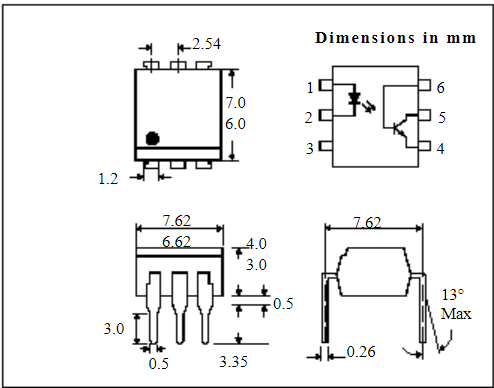
\includegraphics[scale=0.6]{IMG/4N25.png}}
            \subfigure[BC337]{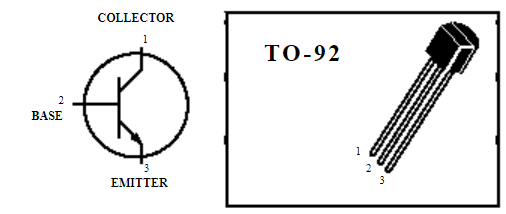
\includegraphics[scale=0.6]{IMG/BC337.png}}
            \caption{Configuracion de las patitas}
            \label{fig:confpat}
        \end{figure}
        \item Se procede a armar la etapa de emicion del circuito siguiendo el digrama dado calculando la resistencia de entrada para regular los 12v y no quemar los optoacopladores y cambiando la resistencia de la salida del transistor dentro del optoacoplador por una de 10k$\Omega$ quedando el circuito como el de la figura 2.\\\\
        $R1=\frac{(V_{en}-V_{carga})}{I}=\frac{12-1.2}{10e^{-3}}=\frac{10.8}{10e^{-3}}=1080K\Omega$\\\\
        Como una resistencia de esta capacidad no es comercial se puede hacer con un potenciometro, ajustandolo a lo requerido, o bien, utilizando una resistencia que se acerque a impedancia requerida.\newpage
        \begin{figure}
            \centering
            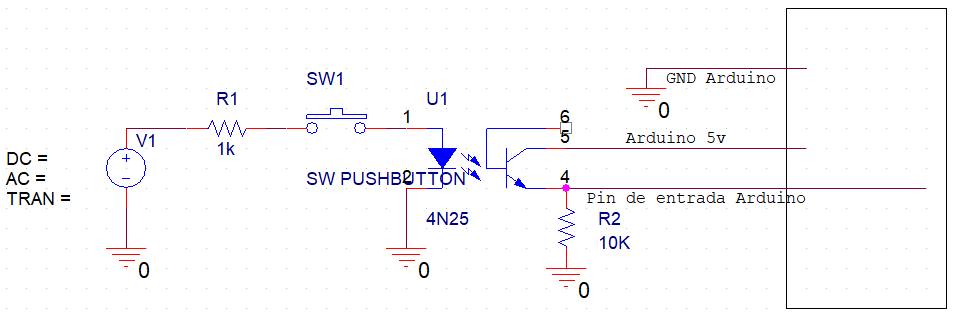
\includegraphics[scale=0.5]{IMG/cir1.png}
            \caption{Circuito de entrada al arduino.}
            \label{fig:cir1}
        \end{figure}
        
        \item Se deben tomar los transistores, ya con la información del data sheet, que nos dice cual es emisor, base y colector, se deben poner en hFe de el multímetro como se ve en la siguiente figura una vez visto el datasheet de nuestro transistor\\
        
        \begin{figure}[htbp]
            \centering
            \subfigure[Opcion hFE]{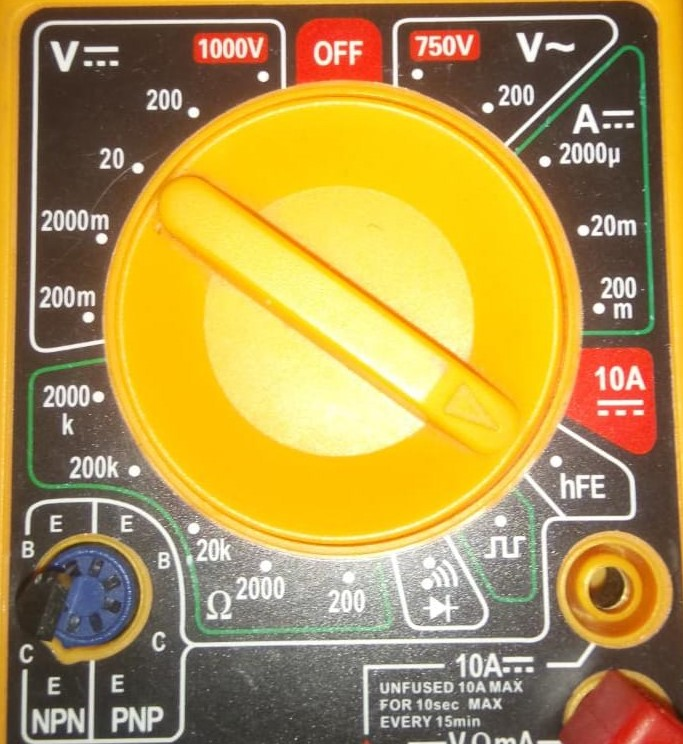
\includegraphics[scale=0.3]{IMG/Mult2.jpeg}}
            \subfigure[Valor de hFE de el BC337 empleado]{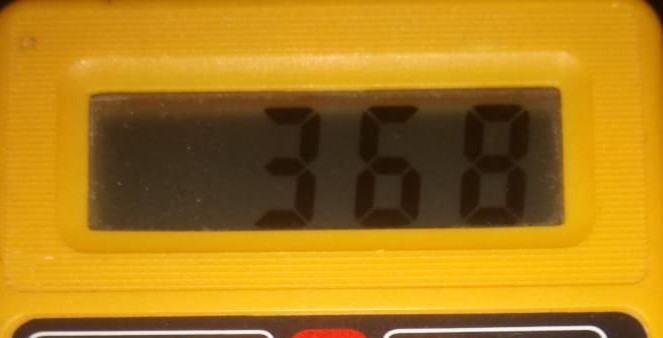
\includegraphics[scale=0.3]{IMG/Mult.jpeg}}
            \caption{Caption}
            \label{fig:my_label}
        \end{figure}
        
        \item Obtenido el hFE de nuestro transistor calculamos la resistencia de base con la formula\\
            \begin{large}
                \begin{center}
                $R = \frac{(V_{in}-0.6)*hFE}{I_{rele}}$ 
                \end{center} 
            
            \end{large}
        \item Ya obtenida la resistencia necesaria para el trancistor se conecta la otra parte del circuito que consiste en un diodo, un led con una resistensia en serie y el relay como se muestra en la figura 4.\\
        \newpage
        \begin{figure}
            \centering
            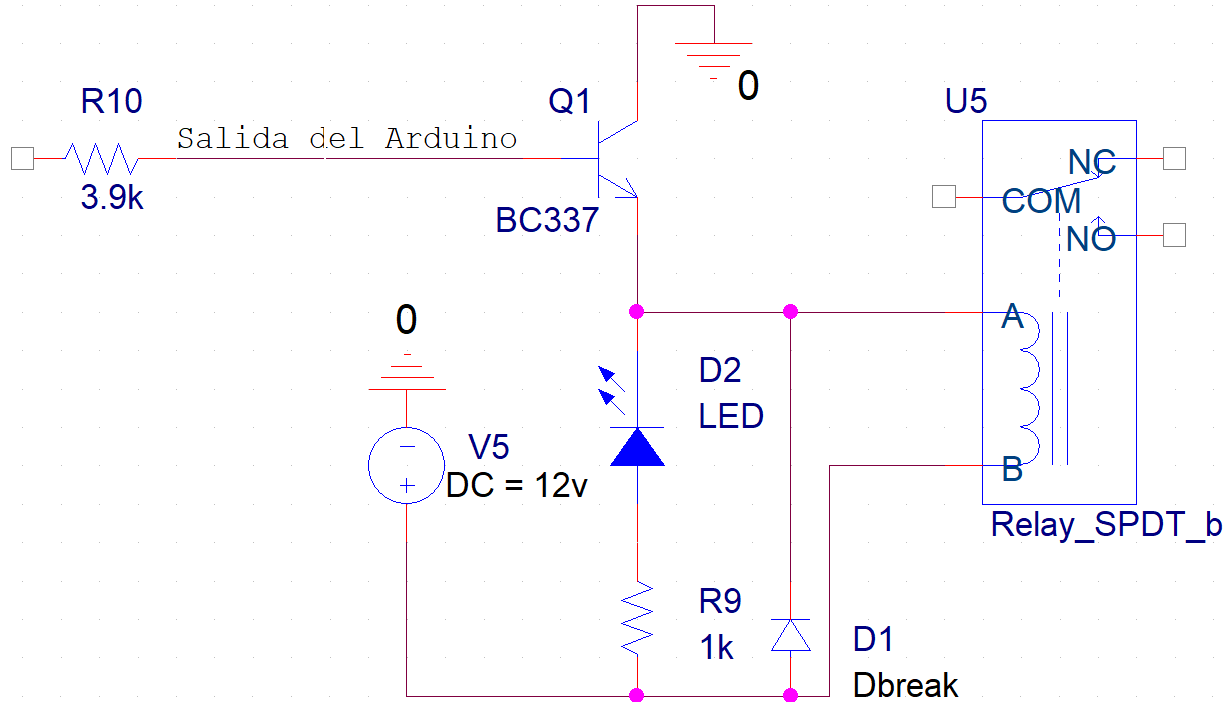
\includegraphics[scale=0.5]{IMG/cir2.png}
            \caption{Segunda parte del circuito principal.}
            \label{fig:cir2}
        \end{figure}
        \item Se conecta al Arduino dependiendo de la programacion previa, para este caso se utilizo el codigo ejemplo de boton en el IDE de Arduino.\\\\
        const int buttonPin = 2;     // the number of the pushbutton pin\\
        const int ledPin =  13;      // the number of the LED pin\\
        \\
        // variables will change:\\
        int buttonState = 0;         // variable for reading the pushbutton status\\
\\
        void setup() {\\
         // initialize the LED pin as an output:\\
         pinMode(ledPin, OUTPUT);\\
         // initialize the pushbutton pin as an input:\\
         pinMode(buttonPin, INPUT);\\
        }\\
\\
        void loop() {\\
            // read the state of the pushbutton value:\\
            buttonState = digitalRead(buttonPin);\\
\\
        // check if the pushbutton is pressed. If it is, the buttonState is HIGH:\\
        if (buttonState == HIGH) {\\
         // turn LED on:\\
         digitalWrite(ledPin, HIGH);\\
        } else {\\
            // turn LED off:\\
            digitalWrite(ledPin, LOW);\\
        }\\
        }\\
        \item Se replican ambas partes del circuito 2 veces mas para finalizar la practica y se modifica el codigo para que pueda recibir mas señales y de igual manera tener más salidas.\\
        Ya replicado el circuito en el esquematica tendria una forma parecida a la de la figura 5.\\
        \begin{figure}[htbp]
            \centering
            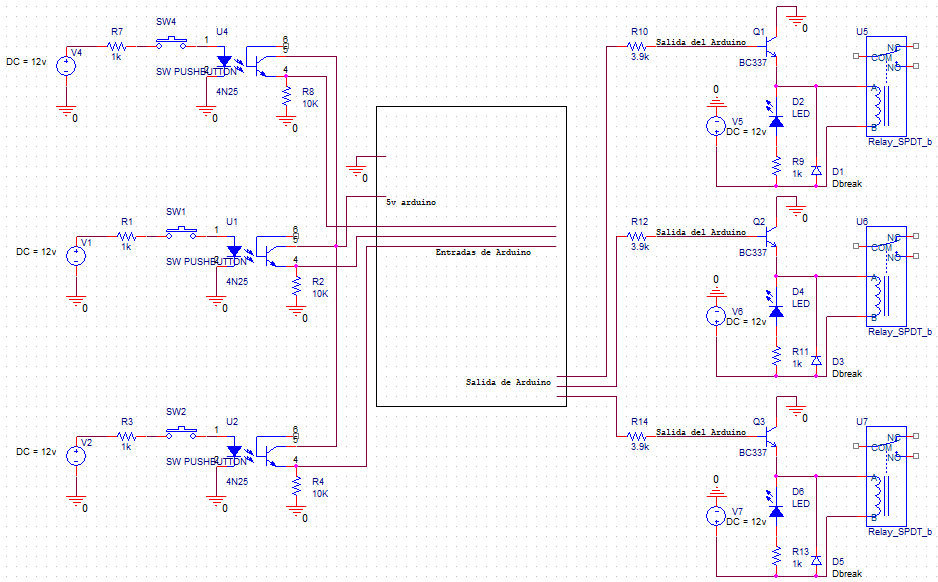
\includegraphics[scale=0.5]{IMG/cir3.png}
            \caption{Circuito completo.}
            \label{fig:cir3}
        \end{figure}
        
        Y el codigo quedaria de la siguiente manera:\\
    Aquí declaramos los pines de entrada de datos\\
const int O1=2; \\
const int O2=3;\\
const int O3=4;\\
Aquí declaramos los pines de salida\\
const int T1=11;\\
const int T2=13;\\
const int T3=10;\\
Declaramos las variables que almacenarán las entradas como dato booleano\\
int VO1 = 0;\\
int VO2 = 0;\\
int VO3 = 0;\\
Comienza diciendo que hará cada pin, si será de entrada o de salida.\\
void setup() {\\
 pinMode(O1, INPUT);\\
 pinMode(O2, INPUT);\\
 pinMode(O3, INPUT);\\
 pinMode(T1, OUTPUT);\\
 pinMode(T2, OUTPUT);\\
 pinMode(T3, OUTPUT);\\
}\\
Decimos a la computadora que guarde la información de los pines en las variables\\
void loop() \{\\
VO1 = digitalRead(O1);\\
VO2 = digitalRead(O2);\\
VO3 = digitalRead(O3);\\

La condición dice, si las variables están en estado 1, es decir botones presionados, el resultado será mandar una señal alta y si no será no mandar señales
if (VO1==HIGH){\\
  digitalWrite(T1, HIGH);\\
}else{\\
  digitalWrite(T1,LOW);\\
if (VO2==HIGH){\\
  digitalWrite(T2,HIGH);\\
}\\
else{\\
  digitalWrite(T2,LOW);\\
}\\
if (VO3==HIGH){\\
  digitalWrite(T3,HIGH);\\
}\\
else{\\
  digitalWrite(T3,LOW);\\
}\\
}
    \end{enumerate}
\end{large}

\newpage
\begin{huge}
    \textbf{Resultados:}\\
\end{huge}
Fueron generadas las condiciones lógicas con base a los elementos dados. Dichos elementos se toman como las partes de un PLC, puesto que hay voltajes de entrada, un proceso que es con el arduino y voltajes de salida que representan las condiciones cumplidas, la práctica siendo par de la materia de \color{cyan}{Controladores lógicos programables}\color{black}, la práctica consta en recibir los resultados de condiciones lógicas con la utilización de Arduino. %leonardo
 \\
 Para este caso la condicion logica que debia seguir Arduino era la de "Seguidor"\\\\
 \begin{figure}[htbp]
     \centering
     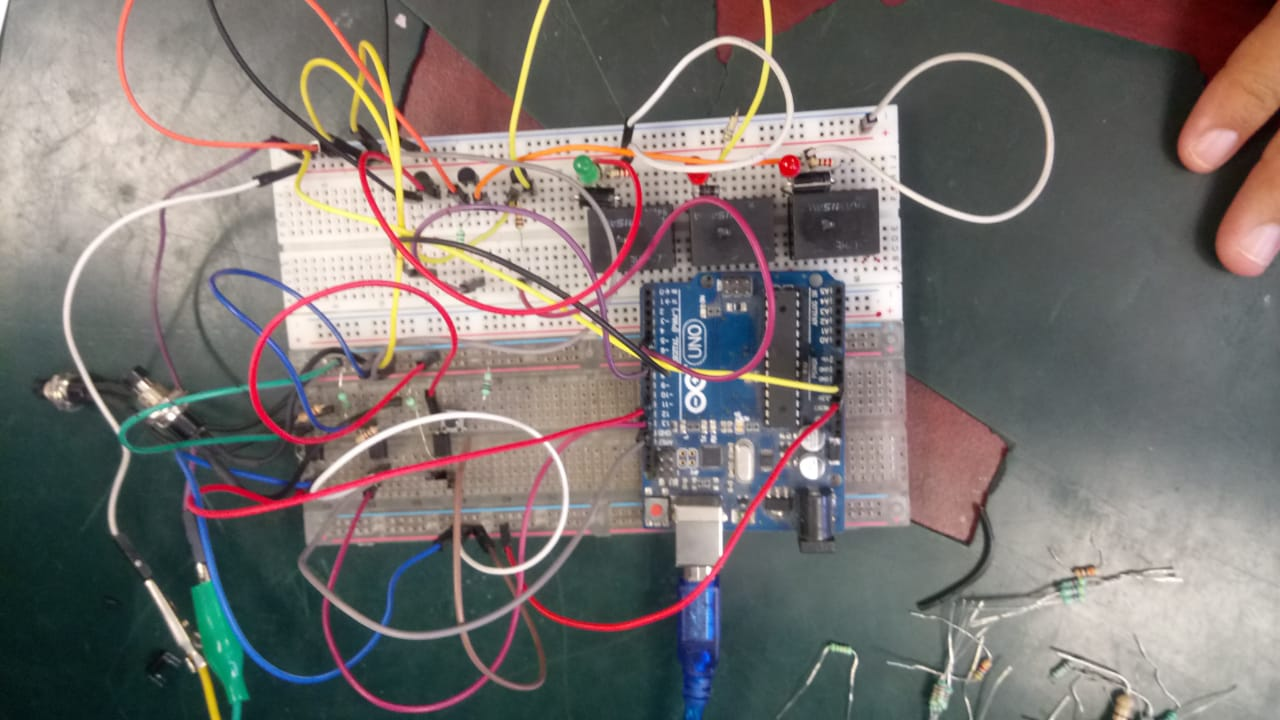
\includegraphics[scale=0.3]{IMG/CirTerm(1).jpeg}
     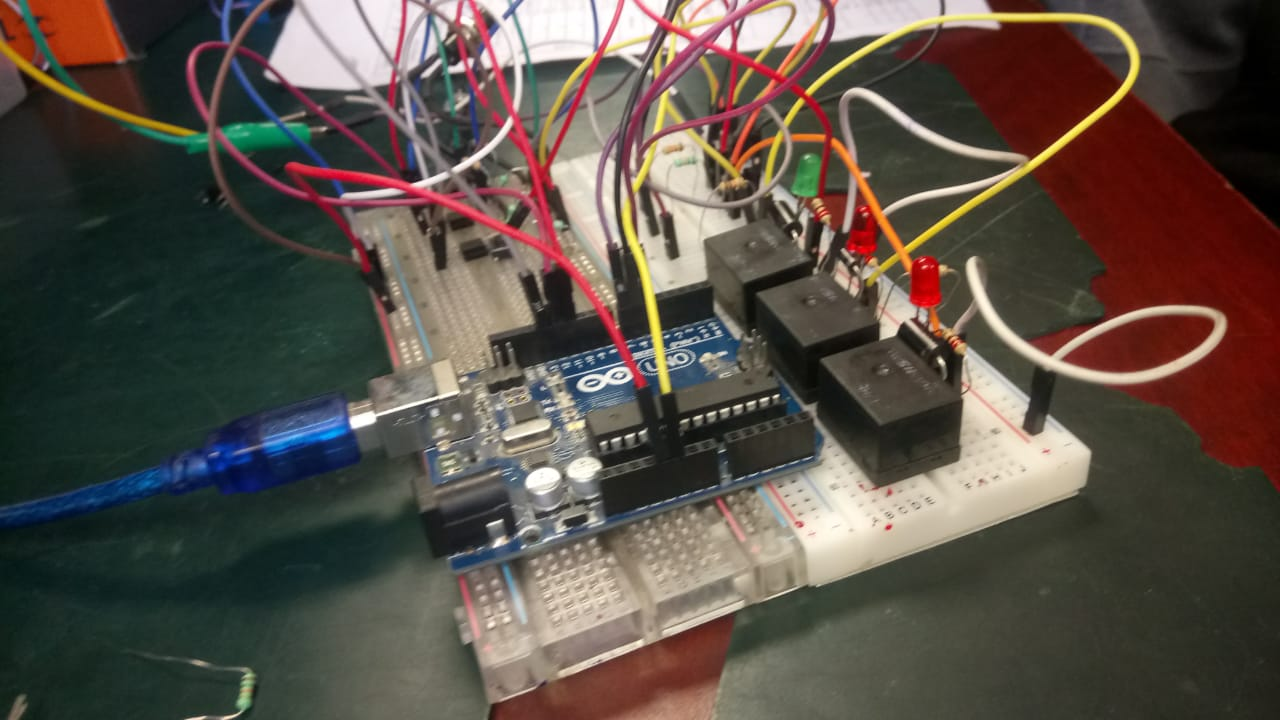
\includegraphics[scale=0.3]{IMG/CirTerm(2).jpeg}
     \caption{Circuito terminado.}
     \label{fig:CirTerm}
 \end{figure}\newpage
 \begin{huge}
    \textbf{Conclusión:}\\
\end{huge}
Dentro de las competencias aprendidas se encuentra la utilización de transistores así como optoacopladores en circuitos con relays, utilizando formulas y metodos de obtención de datos, para la resistencia de la base del transistor asi como la resistencia de entrada de voltaje para evitar que el circuito se queme.\\
Tambien se puede concluir de esto la ventaja que podria suponer un sistema automatizado de este tipo por la versatilidad y gran rango de configuracion a la que podemos acceder mediante la programacion de una de estas piezas pero de igual manera de debe tener cuidado con los microcontroladores ya que asi como son utiles son delicados y pueden dañarse con una gran facilidad.\\
Por otro lado tambien esta la gran utilidad que tienen los componentes en estos casos, en especial los optoacopladores, el microcontrolador y los trancistores teniendo estos ultimos una funcion muy importante al fungir como un tipo de switch que deja pasar la corriente para la activacion de las bobinas en el circuito y el microcontrolador al interpretar los pequeños pulsos enviados por los optoaclopladores.\\

\end{document}
